
\section{Vision, action, and development}

Robots and animals are actors in their environment, not simply passive
observers.  They have the opportunity to examine the world using
causality, by performing probing actions and learning from the
response.  
Tracing chains of causality from motor action to perception
(and back again) is important both to understand how the brain deals
with sensorimotor coordination and to implement those same functions
in an artificial system, such as a humanoid robot.
In this paper, we propose that such causal probing can be arranged in
a developmental sequence leading to a manipulation-driven
representation of objects.  We present results for many important steps
along the way, and describe how they fit in a larger scale implementation.
And we discuss in what sense our artificial implementation is substantially 
in agreement with neuroscience. 


%
\begin{figure}[tb]
\begin{center}
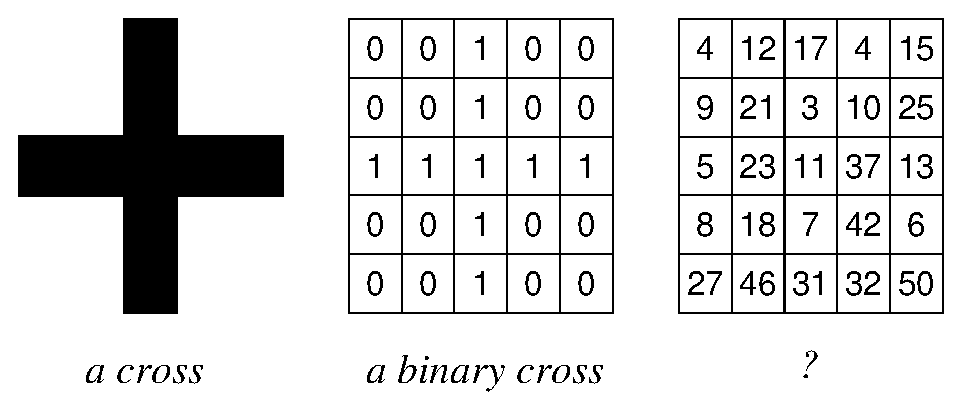
\includegraphics[width=8.0cm]{number-cross.eps}
\hspace{2cm}
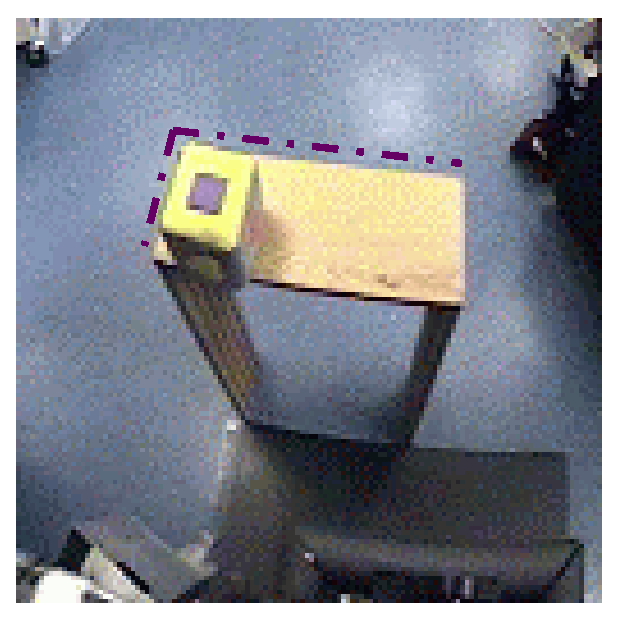
\includegraphics[width=4cm]{setup-sequence.eps}
\caption{ 
\label{fig:number-cross}
%
On the left are three examples of crosses,
following~\cite{manzotti01coscienza}.  The human ability to segment
objects is not general-purpose, and improves with experience.
On the right is an image of a cube on a table, illustrating the
ambiguities that plague machine vision. 
The edges of the table and cube happen to be
aligned (dashed line), the colors of the cube and table are not well
separated, and the cube has a potentially confusing surface pattern.
%
}
\end{center}
\end{figure}
%
%


\ifverbose
\begin{figure}[tbh]
\begin{center}
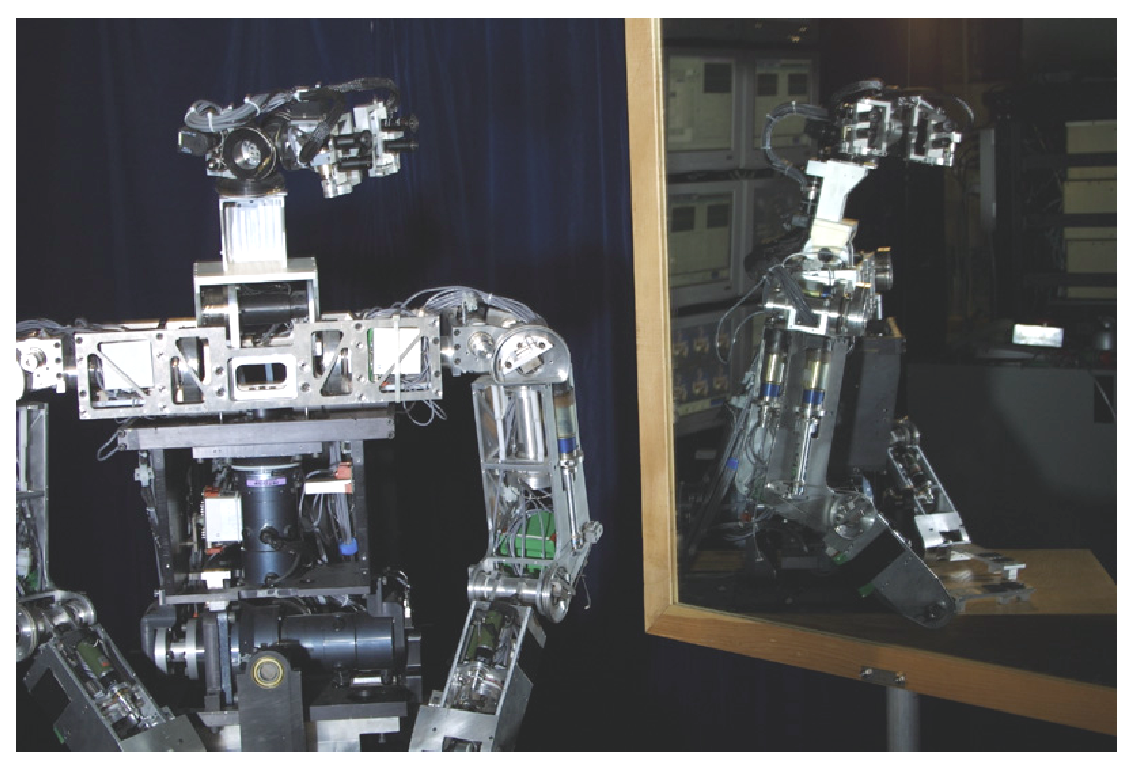
\includegraphics[width=12cm]{mirror-cog.eps}
\caption{ 
\label{fig:mirror-cog}
%
The world is complicated, but contigent.
The ultimate goal of this work is for our robot to follow chains of
causation outwards from its own simple body into the complex world.
Such an incremental process suggests that perception and action
develop together, supporting each other.
%
}
\end{center}
\end{figure}
\fi


%We address three levels of causal complexity.
Table \ref{tab:causation} shows three levels of causal complexity
that we address in the paper.
The simplest causal chain that an actor~-- whether robotic or biological~-- may experience is the
perception of its own actions.  The temporal aspect is immediate:
visual information is tightly synchronized to motor commands.
Once this causal connection is established, we can go further and use
it to actively explore the boundaries of objects.  In this case, there
is one more step in the causal chain, and the temporal nature of
the response may be delayed since initiating a reaching movement doesn't
immediately elicit consequences in the environment.  
Finally we argue that extending this causal chain further will allow
the actor to make a connection between its own actions and the actions 
of another. This is reminiscent of what has been observed in the response
of the monkey's premotor cortex. 

%
% Sounds a bit of an excuse :)
%
% It is, but it is a good one! ;)
%
We wished to keep the actions implemented on our robotic system as
simple as possible, to avoid obscuring the core issue of development
behind an elaborately engineered dextrous system.
%
%
% I wish I had an elaborate dextrous system.
%
%% oh, and Cog's arms suck too, that was another reason :)
%
We found that simple poking gestures
(prodding, tapping, swiping, batting, etc.) were rich enough 
to evoke object affordances such as rolling and to provide
the kind of training data needed to bootstrap perception.


%\ifverbose
\begin{table*}[htbp]
\begin{center}
\begin{tabular}{|p{5.2cm}|p{4.5cm}|p{4.5cm}|}
\hline
{\it type of activity} & {\it nature of causation} &  {\it time profile} \\ \hline\hline
{\bf sensorimotor coordination} & direct causal chain & strict synchrony \\ \hline
{\bf object probing} & one level of indirection & fast onset upon contact, potential for delayed effects\\ \hline
{\bf constructing mirror representation} &  complex causation involving multiple causal chains & arbitrarily delayed onset and effects\\ \hline
\end{tabular}
\caption{
\label{tab:causation}
%
Degrees of causal indirection. There is a natural
trend from simpler to more complicated tasks.  The more time-delayed
an effect, the more difficult it is to model.
%
}
\end{center}
\end{table*}
%\fi

\section{Object or illusion?}

Following \cite{manzotti01coscienza}, we can ask whether macroscopic
objects exist completely in their own right, or instead owe something
of their existence to their interaction with an observer.  
How the world is divided up, and what parts of it we grant status
as objects, says as much about us as about the world around 
us~\cite{hendriksjansen96catching}.
%
%Being a
%physical assemblage is not an intrinsic or primary property, but
%rather it is something that derives from the observer. 
%
For example, would a chair still be a chair if we had a completely different
embodiment? Further, even if a part of the physical world could be
separated out from the background in an objective manner, its function still depends on our
body and skills -- for example, a floppy disk is of
little to one who is computer illiterate, and perhaps can be just regarded as
a clumbsy frisbee or ugly drink coaster.

Consider the example in Figure~\ref{fig:number-cross}. It is
clear that the cross on the left is a cross and does not seem to owe 
its existence to us as observers. The array in the middle for
many of us is still a cross. This would still be the case 
even if we had not developed the concept of number or these particular
graphic symbols to identify numbers. What can we say about the array 
on the right? On a first examination it looks like a random collection
of numbers. But if we are told that the criterion is ``prime numbers 
vs. non-prime'' then a cross can still be identified.
%% (assuming 
%%we can read and understand numbers of course).

%
% Can we have the yellow car on the yellow table instead?
%
On the very right of figure \ref{fig:number-cross} we show a 
cube sitting on the table. While humans are very good in analyzing
scenes like this one, there are many features that can fool
a computer vision system. The edges of the cube and table 
happen to be aligned, the color is poorly separated, and the surface
pattern of the cube does not really tell much about the object
itself. Is the internal dark square a different object lying on 
top of the cube? Another possibility is that the cube is extremely
heavy or even part of the table and thus it is not manipulable or
movable. Does it make sense then to speak about objects in images,
as if there were a unique correspondence between the two?
%We propose that a possible way to find out for sure is to take 
%actions and test by ourselves. 
As early as 1734, Berkeley observed that:
%
\begin{quote}
...objects can only be known by
touch. Vision is subject to illusions, which arise from the
distance-size problem... \cite{berkeley72new}
\end{quote}
%
Vision is indeed subject to many illusions.  But touch also can be
fooled since it has been shown that vision and touch combine 
optimally with respect to a maximum likelihood criterion 
\cite{ernst-banks-2002}. Which sensory modality dominates 
depends on the experimental conditions and apparently we 
shouldn't always ``blindly'' trust our senses.
% is the 'blindly' ok? 
The key to resolving ambiguity is to take action, rather than remain
a passive observer.
%usually be avoided if we are allowed to take actions. 
%It would be
%also more general to consider action rather than touch only. It 
%has been shown that touch itself can be fooled by vision \cite{}.
In the remainder of the paper we argue that in the presence of
manipulation -- even a simple form of manipulation -- vision 
becomes more powerful and many of its illusions fade away.



\ifverbose 
%% Shall we leave this section for the other paper? --paulfitz

\section{The elusive object}

\label{sect:introduction}

Sensory information is intrinsically ambiguous, and very distant from
the world of well-defined objects in which humans believe they live.  
What criterion should be applied to distinguish one object from
another?  How can perception support such a phenomenon as figure-ground
segmentation?  
Consider the example in Figure~\ref{fig:number-cross}.  It is
immediately clear that the drawing on the left is a cross, perhaps
because we already have a criterion, which allows segmenting on the
basis of the intensity difference. It is slightly less clear that the
zeros and ones int the first grid are still a cross. What can we say
about the second grid? If we are not told, and we do not have
the criterion to perform the figure-ground segmentation, we might
think this is just a random collection of numbers. But if we are told
that the criterion is ``prime numbers vs. non-prime'' then a cross can
still be identified.

While we have to be inventive to come up with a segmentation problem
that tests a human, we don't have to go far at all to find something
that baffles our robots.  Figure~\ref{fig:number-cross} (right) shows a
robot's-eye view of a cube sitting on a table.  Simple enough, but
many rules of thumb used in segmentation fail in this particular case.
And even an experienced human observer, diagnosing the cube as a
separate object based on its shadow and subtle differences in the
surface texture of the cube and table, could in fact be mistaken --
perhaps some malicious researcher is up to mischief.  The only way to
find out for sure is to take action, and start poking and prodding.
As early as 1734, Berkeley observed that:
%
\begin{quote}
...objects can only be known by
touch. Vision is subject to illusions, which arise from the
distance-size problem... \cite{berkeley72new}
\end{quote}
%
In this paper, we provide support for a more nuanced proposition: that
in the presence of physical contact, vision becomes more powerful, and many of
its illusions fade away.


%
\begin{figure}[tb]
\begin{center}
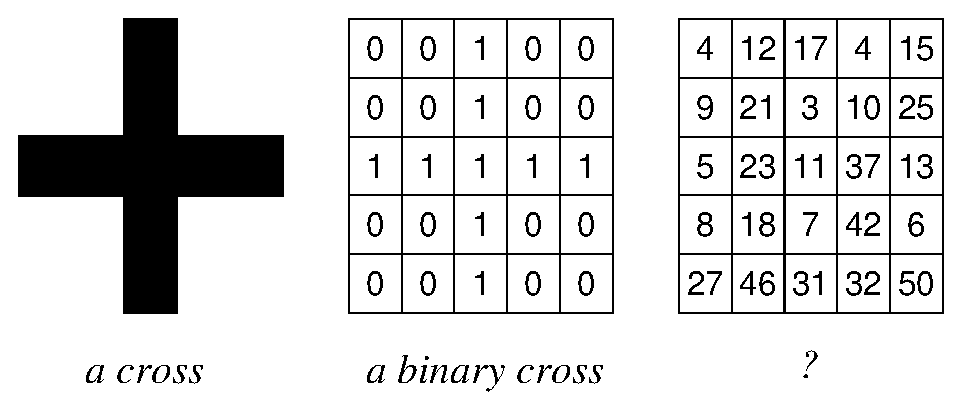
\includegraphics[width=8.0cm]{number-cross.eps}
\hspace{2cm}
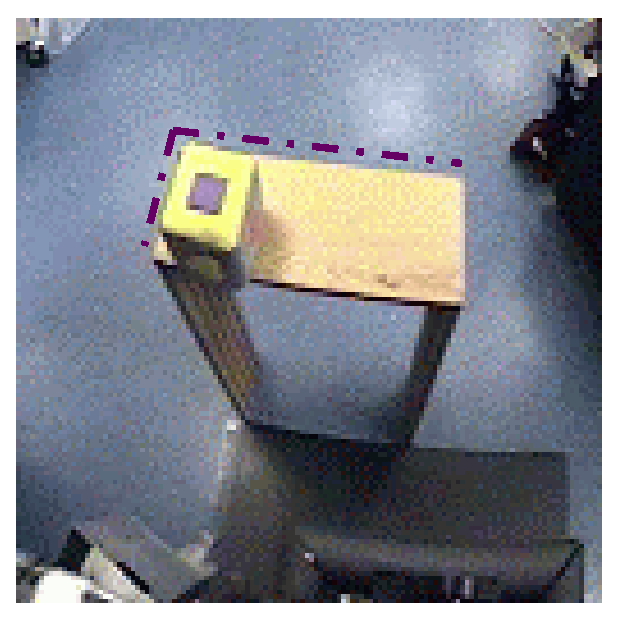
\includegraphics[width=4cm]{setup-sequence.eps}
\caption{ 
\label{fig:number-cross}
%
On the left are three examples of crosses,
following~\cite{manzotti01coscienza}.  The human ability to segment
objects is not general-purpose, and improves with experience.
On the right is an image of a cube on a table, illustrating the
ambiguities that plague machine vision. 
The edges of the table and cube happen to be
aligned (dashed line), the colors of the cube and table are not well
separated, and the cube has a potentially confusing surface pattern.
%
}
\end{center}
\end{figure}
%
%

\fi



%
%
%

\section{Objects and action in humans}
\label{sec:humans}

%%\subsubsection*{Objects and actions}

%\ifverbose
The example of the cross composed of prime numbers is a novel (albeit
unlikely) type of segmentation in our experience as adult humans.  We
might imagine that when we were very young, we had to initially form a
set of such criteria to solve the object identification/segmentation
problem in more mundane circumstances. 
%\else
%Humans are experts at solving the figure/ground problem, and
%segmenting objects out from their background.
%\fi
%
That such abilities
develop and are not completely innate is suggested by results in
neural science. For example Kovacs~\cite{kovacs00human} has shown that
perceptual grouping is slow to develop and continues to improve well
beyond early childhood (14 years). Long-range contour integration was
tested and this work elucidated how this ability develops to enable
extended spatial grouping.

\ifverbose
The pattern of interconnections in the visual cortex is also known
to complete development postnatally from cell staining methods
studies~\cite{burkhalter93development,callaway92development}.
Brown~\cite{brown94vision} argued that a developmental process, that
is one of structure formation, is involved in acquiring visual
abilities rather than a pure parameter adaptation procedure as in
machine learning algorithm.
\fi 

%Key to understanding how such capabilities could develop is the
A useful concept to understand how such capabilities could develop is the
well-known theory of Ungerleider and Mishkin~\cite{ungerleider82two}
\ifrev
who first formulated the hypothesis that the brain's visual pathways 
split into two main streams: the dorsal and the ventral. The dorsal is 
the so-called ``where'' pathway, concerned with the analysis of the
spatial aspects of motor control. The ventral is related with
the ``what'', i.e. the identity of objects.

Goodale and Milner~\cite{milner95visual} refined the theory by proposing
that objects are represented differently during action than they are 
for a purely perceptual task. The dorsal deals with the information required 
for action, while the ventral is important for more cognitive tasks such 
as maintaining an object's identity and constancy.  
\else
who first formulated the hypothesis that objects are represented
differently during action than they are for a purely perceptual task.
Briefly, they argue that the brain's visual pathways split into two
main streams: the dorsal and the ventral~\cite{milner95visual}. The
dorsal deals with the information required for action, while the
ventral is important for more cognitive tasks such as maintaining an
object's identity and constancy.  
\fi
Although the dorsal/ventral
segregation is emphasized by many commentators, it is significant that
there is a great deal of cross talk between the streams.  Observation
of agnosic patients~\cite{jeannerod97cognitive} shows a much more
complicated relationship than the simple dorsal/ventral dichotomy
would suggest.  For example, although some patients could not grasp
generic objects (e.g.  cylinders), they could correctly preshape the
hand to grasp known objects (e.g. a lipstick): interpreted in terms of
the two pathways, this implies that the ventral representation of the
object can supply the dorsal stream with size information.

%
%
\begin{figure}[tb]
\begin{center}
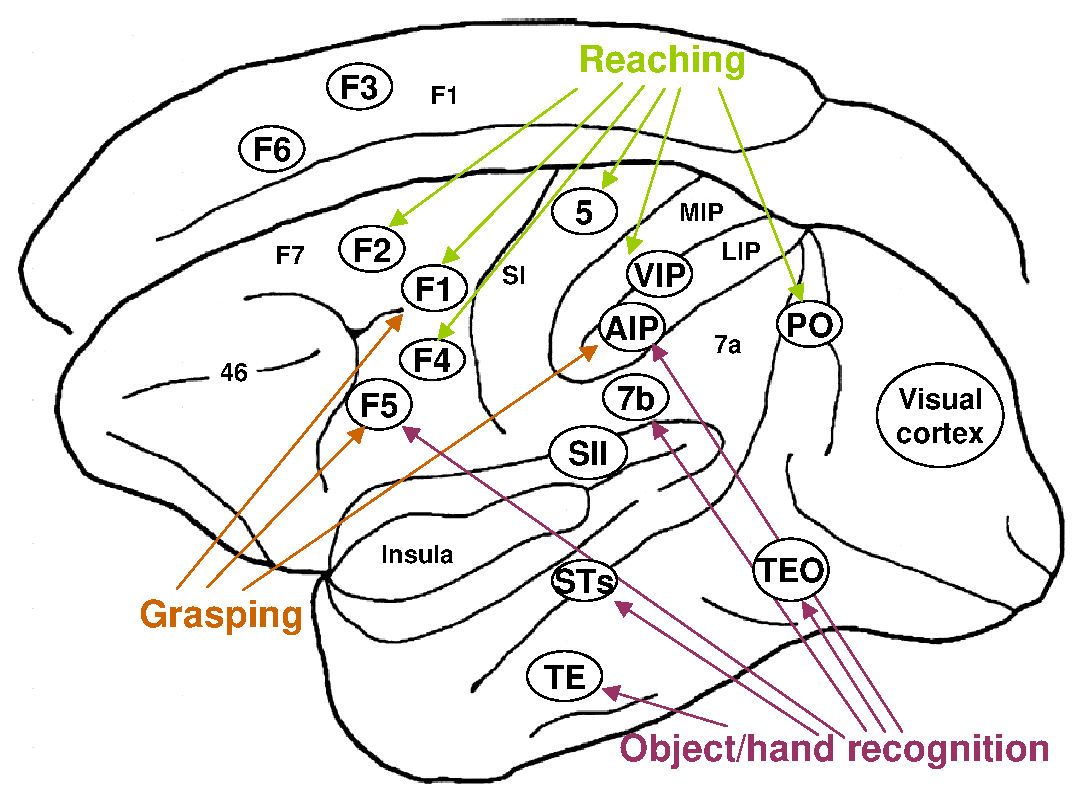
\includegraphics[width=10cm]{brain-schema2.eps}
%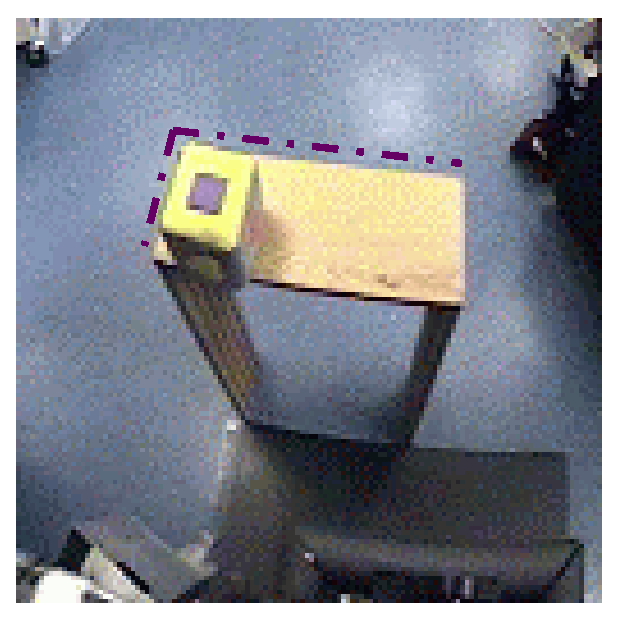
\includegraphics[width=\columnwidth]{setup-sequence.eps}
%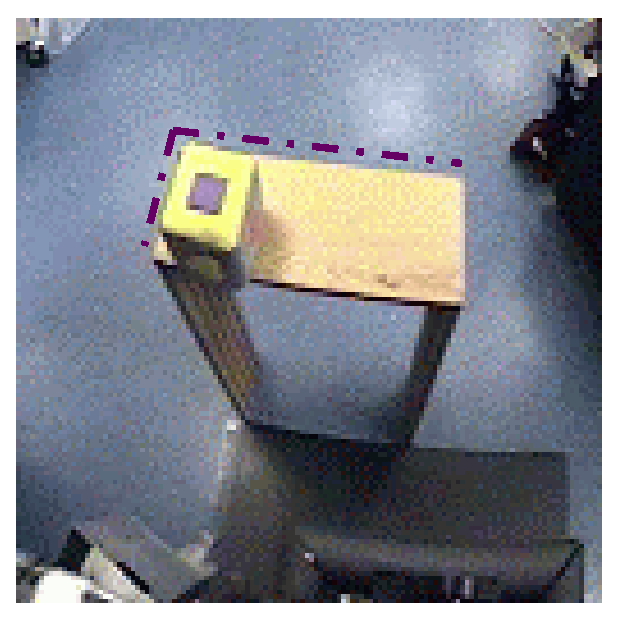
\psfig{file=setup-sequence.eps,width=4cm}
\caption{ 
\label{fig:brain-schema}
%
Monkey brain with indication of the main areas participating in object
oriented actions (adapted from~\cite{fagg-arbib-1998}). As described in the
text, three main functions can be identified: object recognition, reaching,
and grasping. These form three parallel yet connected streams of 
processing. The circuit connecting the visual cortex to the inferior parietal 
lobule VIP, F4 and F1 is thought to compute the visuomotor
transformations required to control reaching. Some evidence also suggests
a possible role in the organization of reaching played by the posterior
parietal cortex PO and dorsal premotor area F2, reciprocally connected.
AIP and F5 are responsible for grasping. Temporal areas (TE, TEO) and STs 
are correlated to the semantic of object recognition.
%
% If we need to ask permission, I guess that's for the final version anyway
}
\end{center}
\end{figure}
%
%

Grossly simplifying, the brain circuitry responsible 
for object oriented actions is thought to consist of at least four 
interacting regions (Figure~\ref{fig:brain-schema}), namely the primary motor cortex (F1), the premotor cortex (F4, F5), the 
inferior parietal lobule (AIP, VIP), and the temporal cortex 
(TE, TEO)~(see \cite{rizzolatti-fogassi-gallese-1997,fadiga00visuomotor,jeannerod97cognitive} 
for a review). 
While this is a useful subdivision, it is worth bearing in mind 
that the connectivity of the brain is much more complex, that bidirectional 
connections are present, and that behavior is the result of a 
population activity of these areas. The example about the grasping of known 
objects in agnosic patients testifies to the \emph{abundance of anatomical connections} 
between different regions \cite{jeannerod-arbib-rizzolatti-sakata-1995}.

Another way of looking at the same connectivity is in terms of the main 
function of each area. For example F4, VIP, and 7b are involved in the control of 
reaching, F5 and AIP contain the majority of grasp related neurons, 
while TE and TEO are thought to subserve object recognition. These regions together form a network 
of parallel and yet interacting processes. In fact, at the behavioral level, it has 
been observed that reaching and 
grasping need to interact to correctly orient and preshape the hand~\cite{jeannerod-arbib-rizzolatti-sakata-1995}.

Neurons responsive to reaching are present in the inferior parietal lobule. For 
example, Jeannerod et al. reported 
that the temporary inactivation of the caudal part (VIP) of the intraparietal sulcus by injecting a GABA 
agonist
disrupts reaching~\cite{jeannerod-arbib-rizzolatti-sakata-1995}. Conversely, injection in the more rostral part (area AIP) 
interferes with the
preshaping of the hand. 

Some of the VIP neurons have bimodal visual and somatic receptive 
fields (RF). About 30\% of them have a RF which does not vary with 
movement of the head~\cite{rizzolatti-fogassi-gallese-1997}. The tactile and 
visual RF often overlap (e.g. a central visual 
RF corresponds to a tactile RF in the nose or mouth). The parietal cortex also contains 
cells related to eye position/movements that appear to be involved in  
the visuo-motor transformation required for reaching. VIP projects to area 
F4 in the premotor cortex. Area F4 contains neurons that respond to objects and 
are related to the description of the peripersonal space with respect to reaching~\cite{graziano-hu-gross-1997,fogassi96coding}. A subset of the F4 neurons 
have a somatosensory, visual, and motor receptive field. The visual receptive 
field extends in 3D from a given body part, such as the forearm. The somatosensory RF
is usually in register with the visual one (as in VIP neurons). Motor information
is integrated into the representation by maintaining the receptive
field anchored to the correspondent body part (the forearm in this
example) irrespective of the relative position of the head and arm.

Also, Graziano et al.~\cite{graziano-hu-gross-1997a} described neurons that maintain a 
memory of the position of objects for the purpose of reaching. They found neurons 
that change their firing rate after an object is illuminated briefly
within reaching distance. The neurons return 
to their baseline firing rate only after the monkey is shown that the object have been 
taken away or moved to a different position.

Sakata and coworkers~\cite{sakata-taira-kusunoki-murata-tanaka-1997} 
investigated the response of neurons in the 
parietal cortex and in particular in area AIP (anterior intra-parietal). They found 
cells responsive to complex visual stimuli. Neurons in AIP responded during 
grasping/manipulative actions and when an object was presented to the 
monkey but no reaching was allowed. Neurons were classified as motor dominant, 
visual dominant or visuo-motor type depending on how they fired in the dark. Of 
the visual dominant neurons, some responded to the presentation of the 
object alone and often they were very specific to the size and orientation of the 
object, others to the type of object, while yet others responded indifferently to the 
presentation of a broad class of objects. Area AIP is interesting because 
it contains both motor and visually responsive cells intermixed in various proportions; 
it can be thought of as a visuo-motor vocabulary for controlling object directed 
actions. It is also interesting because projections from AIP terminate in the 
agranular frontal cortex. For many years, because of the paucity of data, this 
part of the cortex was considered a unitary motor control area. Recent studies 
(see~\cite{jeannerod97cognitive,fadiga00visuomotor}) have demonstrated 
that this is not the case. Particularly surprising was the discovery of visual 
responsive neurons. A good proportion of them have both visual/sensory and motor 
responses. Area F5, one of the main targets of the projection from AIP (to which 
it sends back recurrent connections), was thoroughly investigated by Rizzolatti 
and colleagues~\cite{gallese-fadiga-fogassi-rizzolatti-1996}.

%
%
\ifverbose
The dorsal stream goes through the parietal lobe and premotor cortex,
which project heavily onto the primary motor cortex to eventually
control movements. For many years the premotor cortex was considered
just another big motor area.  Recent studies~\cite{jeannerod97cognitive} have demonstrated that this is not the
case.  Visually responsive neurons have been found: some are purely
visual, but many have significant visuo-motor characteristics. In area
F5 in the monkey, neurons responding to object manipulation gestures
are found.  
\fi

F5 neurons can be classified in at least two different categories:
canonical and mirror.
%% (see Figure~\ref{fig:canonical-mirror}). 
Canonical and mirror neurons are 
indistinguishable from each other on the basis of their motor responses; 
their visual responses however are quite different. 
The canonical type is active in two situations:
i) when grasping an object and ii) when fixating that same object.
For example, a neuron active when grasping a ring also fires when the
monkey simply looks at the ring.  This could be thought of as a neural
analogue of the ``affordances'' of Gibson~\cite{gibson77theory}. 
However, given the heavy projection from AIP, it is not entirely
true that the affordances are fully described/computed by F5 alone.
A more conservative stance is that the system of AIP, F5, and other areas 
(such as TE) participate in the visual processing and motor matching required 
to compute the affordances of a given object.  

\ifverbose
\begin{figure}[tbh]
\begin{center}
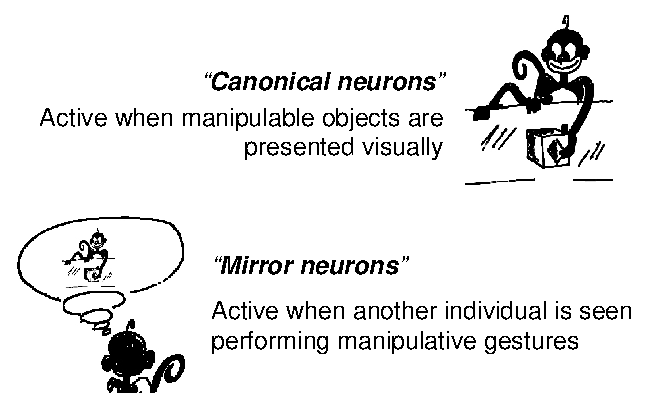
\includegraphics[width=10cm]{fig-canonical-mirror.eps}
\caption{ 
\label{fig:canonical-mirror}
%
Canonical and mirror neurons.
%
}
\end{center}
\end{figure}
\fi


\ifverbose
%
The affordances are a pragmatic action-related description of objects:
they can be seen as the properties of an object that can be exploited
by action.  For example a coffee mug has certainly a full palm
grasping affordance but also a precision grip one if using the handle
to lift it.
%
\fi

The second type of neuron identified in F5, the mirror neuron~\cite{fadiga00visuomotor}, becomes active under either of two conditions: i)
when manipulating an object (e.g. grasping it, as for canonical neurons), and ii) when watching
someone else performing the same action on the same object. This is a
more subtle representation of objects, which allows and supports, at
least in theory, mimicry behaviors. In humans, area F5 is thought to
correspond to Broca's area; there is an intriguing link between
gesture understanding, language, imitation, and mirror neurons~\cite{rizzolatti98language}.

The superior temporal sulcus region (STs) and parts of TE contain neurons
that are similar in response to mirror neurons~\cite{perret-mistlin-harries-chitty-1990}. 
They respond to the sight of the hand; the main difference compared to F5
is that they lack the motor response. It is likely that they participate in the 
processing of the visual information and then communicate with 
F5~\cite{gallese-fadiga-fogassi-rizzolatti-1996} most likely via the parietal
cortex.

\ifrev
A possible developmental explanation of the acquisition of
these functions can be framed in terms of tracing/interpreting chains 
of causally related events. The ability to probe longer chains 
triggers the emergence of new functionality and/or a new set of behaviors. 
The next sections delves deeper into this proposal for the ontogenesis of 
object oriented action and provides experimental results of many steps
towards this goal.
\else
A possible developmental explanation of the acquisition of
these functions can be framed in terms of tracing/interpreting chains 
of causally related events. Although it is still speculative, this analysis 
predicts that i) development of functions roughly follows a dorsal to ventral 
temporal gradient (i.e. reaching, grasping, recognition); ii) the 
ability to probe longer chains triggers the emergence of new functionality 
and/or a new set of behaviors. 
The next section delves deeper into
this proposal for the ontogenesis of object oriented action and
provides a hypothesis amenable to implementation.
\fi

\ifverbose
Also, looking at the three examples, we can notice 
a trend in complexity, and consequently we can hypothesize, that the time 
required to reach proficiency in each task is proportional to this complexity.
\fi

\ifverbose
Another important class of neurons in premotor cortex is found in area
F4~\cite{fogassi96coding}. While F5 is more concerned with the distal
muscles (i.e. the hand), F4 controls more proximal muscles (i.e.
reaching). A subset of neurons in F4 has a somatosensory, visual, and
motor receptive field. The visual receptive field (RF) extends in 3D
from a given body part, for example, the forearm. The somatosensory RF
is usually in register with the visual one. Finally, motor information
is integrated into the representation by maintaining the receptive
field anchored to the correspondent body part (the forearm in this
example) irrespective of the relative position of the head and arm.
\fi







\section{A working hypothesis}

%%In particular, for the problem of getting an operational 
%%definition of object, it seems that action is a necessary component.
%%Taken together, these results from neuroscience suggest that relating
%%motor action to visual perception is fruitful.  

Taken together these results from neuroscience suggest a critical role
for motor action in perception. Certainly vision and action are
intertwined at a very basic level.  While an
experienced adult can interpret visual scenes perfectly well without
acting upon them, linking action and perception seems crucial to the
developmental process that leads to that competence.  We can construct
a working hypothesis: that action is required for object recognition in
cases where an agent has to develop categorization autonomously. 
Of course in standard supervised learning action is not required since
the trainer does the job of pre-segmenting the data by hand.  In an
ecological context, some other mechanism has to be provided.
Ultimately this mechanism is the body itself that through action
(under some suitable developmental rule) generates informative
percepts.

We can distinguish three main conceptual functions (similar to the 
schema of Arbib et al. \cite{arbib-1981}): reaching, grasping (manipulation), and
object recognition. These functions correspond to the three levels of causal understanding introduced in Table~\ref{tab:causation}.
They also form also an elegant progression of abilities which emerge out
of very few initial assumptions. All that is required is the 
interaction betweeen the actor and the environment, and a set of appropriate
developmental rules specifying what information is retained during the
interaction, the nature of the sensory processing, the range of motor
primitives, etc. 
%
The neuroscience results outlined in the previous section can be streamlined
into a developmental sequence roughly following a dorsal to ventral
gradient. Unfortunately this is a question which has not yet been investigated in detail
by neuroscientists, and there is very little empirical support for this claim
(beside the work of Kovacs et al. \cite{kovacs00human}).

What is certainly true is that the three modules/functions can be 
clearly identified. If our hypothesis is correct then 
the first developmental step has to be that of transporting the hand 
close to the object. In humans, this function is accomplished mostly by the
circuit VIP/LIP/7b-F4-F1. Reaching requires at least the detection of
the object and hand, and the transformation of their positions into appropriate 
motor commands. Parietal neurons seem to be coding for the spatial
position of the object in non-retinotopic coordinates by taking
into account the position of the eyes with respect to the head. 
According to \cite{pouget-ducom-torri-bavelier-2002} and 
to \cite{flanders-daghestani-berthoz-1999} the 
gaze direction (the eye motor plant) seems to be the privileged
reference system used to code reaching. 
Relating to the description of causality, the link between an executed
motor action and its visual consequences can be easily formed by 
a subsystem that can detect causality in a short time frame (the immediate
aspect).


Once reaching is reliable enough, we can start to move our attention 
outwards onto objects. Area AIP and F5 are involved in the
control of grasping and manipulation. F5 talks to the 
primary motor cortex for the fine control of movement. 
The AIP-F5 system responds to the ``affordances'' of the observed 
object with respect to the
current abilities.
% (for a robotic implementation,
%these may be simply poking and prodding initially). 
Arbib and coworkers \cite{fagg-arbib-1998} proposed 
the FARS model as a possible description of the computation in AIP/F5. 
They did not however consider how affordances can be 
actually learned during interaction with the environment. 
Learning and understanding affordances requires a slightly longer 
time frame since the initiation of an action (motor command) does not
immediately elicit a sensory consequence. In this example, the initiation
of reaching requires a mechanism to detect when an object is actually 
touched, manipulated, and whether the collision/touch is causal to the
initiation of the movement.

The next step along this hypothetical developmental route is to 
acquire the F5 mirror representation. We might think of canonical neurons as
an association table of grasp/manipulation (action) types with object
(vision) types.  Mirror neurons can then be thought of as a 
second-level associative map which links together the observation of 
a manipulative action performed by somebody else with the neural 
representation of one's own action.
Mirror neurons bring us to an even higher level of causal 
understanding. In this case the action execution has to be associated
with a similar action executed by somebody else. The two events
do not need to be temporally close to each other. Arbitrary time delays
might occur.

The conditions for when this is feasible are a consequence of active
manipulation. During a manipulative act there are a number of
additional constraints that can be factored in to simplify
perception/computation.  For example, detection of useful events is
simplified by information from touch, by timing information 
about when
reaching started, and from a knowledge of the location of the object.% in
%the first place.

The last subsystem to develop is object recognition. Object 
recognition can build on manipulation in finding the boundaries
of objects and segmenting them from the background. More importantly,
once the same object is manipulated many times the brain can
start learning about the criteria to identify the object if 
it happens to see it again. These functions are
carried out by the infero-temporal cortex (IT).
The same considerations apply to the recognition of the 
manipulator (either one's own, or another's). In fact, the STs region is specialized
for this task. Information about object identity is
also sent to the parietal cortex and contributes to 
the formation of the affordances. 
%%
%For the actual recognition we 
%can resort to a fuzzier definition
%of causality where multiple instances of manipulation on a 
%certain object need to be grouped together. That is, all the 
%information (visual in this case) pertaining to a certain object
%has to be grouped (and stored somewhere/somehow) to build a model of some sort
%of the object.
However object recognition is performed, at a minimum all information (visual in this case) pertaining to a certain object
needs to be grouped during development so that a model of the object can be constructed.

\begin{table*}[htbp]
\begin{center}
\begin{tabular}{|p{3.5cm}|p{2.5cm}|p{4.5cm}|}
\hline
{\it nature of causation} & {\it main path} &  {\it function and/or behavior} \\ \hline\hline
{\bf direct causal chain} & VC-VIP/LIP/7b-F4-F1 & reaching\\ \hline
{\bf one level of indirection} & VC-AIP-F5-F1 & poking, prodding, grasping\\ \hline
{\bf complex causation involving multiple causal chains} & VC-AIP-F5-F1+STs+IT & mirror neurons, mimicry\\ \hline
{\bf complex causation involving multiple instances of manipulative acts} & STs+TE-TEO & object recognition\\ \hline
\end{tabular}
\caption{
\label{tab:circuits}
%
Degrees of causal indirection, localization and function in the brain.
%
}
\end{center}
\end{table*}

For the robotic implementation we endeavor to follow the same developmental
pathway and exploit the same sort of causal links between actions and 
sensory feedback.

